%
% empilhamento.tex (LateX)
% 
% Objetivo: Capítulo sobre a etapa de modelagem do relatório de qualificação de doutorado.
% 
% Versão 1.0
% 
% Site: http://www.dirackslounge.online
% 
% Programador: Rodolfo A. C. Neves (Dirack) 17/10/2019
% 
% Email: rodolfo_profissional@hotmail.com
% 
% Licença: GPL-3.0 <https://www.gnu.org/licenses/gpl-3.0.txt>.

\chapter{EMPILHAMENTO FAMÍLIAS ERC}

O empilhamento ERC foi realizado após a interpolação com filtros adaptativos de predição de erro (FPE). Esta etapa de
interpolação permite amostrar a trajetória de tempo de trânsito ERC com um intervalo de amostragem satisfatório no
domínio do PMC. O empilhamento ERC é feito nas famílias ERC sobre as trajtórias de tempo de trânsito ERC. Cada ponto sobre
a seção empilhada ERC (m0,t0) corresponderá a uma família ERC e a uma trajetória ERC, o resultado do empilhamento no domínio
ERC é atribuído à coordenada m0,t0 na seção empilhada ERC, formando a imagem na seção empilhada.

Para demonstrar o funcionamento do empilhamento ERC, selecionamos um único traço na coordenada $m_0=4Km$ no modelo do refletor
gaussiano no Capítulo 5. O espectro de amplitude deste traço é apresentado na Figura \ref{fig:7.1}, o máximo valor de amplitude 
está na frequência 10Hz e corresponde a frequência pico da wavelet utilizada.


Foi realizada a interpolação FPE para o cubo de dados do modelo do refletor gaussiano (vide Capítulo 5), aumentando a amostragem
do modelo na corrdenada do PMC para 802 PMC's, e diminuindo a discretização para 0.0125Km também no domínio PMC. O processo 
de interpolação seleciona as seções de afastamento constante no cubo de dados, intercala os traços originais da seção com traços 
zerados e interpola os traços intercalados utilizando a informação dos traços originais. Este processo é feito para cada seção
de afastamento constante selecionada, regularizando todo o cubo de dados.

Para obter o supertraço empilhado do PMC escolhido ($m_0=4$) é escolhida uma janela de tempo $0<t_0<1$, e para cada par $m_0,t_0$
são calculados os parâmetros do SRC de afastamento nulo $R_{NIP}$ e $\beta_0$ através da otimização global com o Very Fast
Simulated Aneeling (VFSA). Após a obtenção dos parâmetros ótimos, deteminamos as coordenadas $m,h$ que fazem parte da trajetória ERC
e buscamos no cubo de dados interpolados os traços que estão sobre esta trajetória, estes formam uma família ERC.

Os parâmetros $R_{NIP}$ e $\beta_0$ também permitem calcular uma trajetória de empilhamento no domínio ERC, esta será utilizada
para empilhar as amostras sobre esta curva na família ERC correspondente a uma coordenada $m_0, t_0$ da seção empilhada.
Cada $m_0$ constante corresponde a um supertraço da seção empilhada ERC. 

A Figura \ref{fig:7.2} apresenta o resultado do empilhamento para o supertraço $m_0=4Km$. O supertraço apresenta ruído numérico
proveninte dos processos de interpolação e empilhamento, para atenuar este ruído utilizamos um filtro banda-passante no 
intervalo de 0Hz a 10Hz. O resultado, após a aplicação do filtro, é apresentado na Figura \ref{fig:7.4}. O espectro de amplitudes
do supertraço antes e depois da filtragem é apresentado nas Figuras \ref{fig:7.3} e \ref{fig:7.5}.

\begin{figure}
\caption{Espectro original do traço na seção de afastamento nulo com PMC 4Km.}
\begin{center}
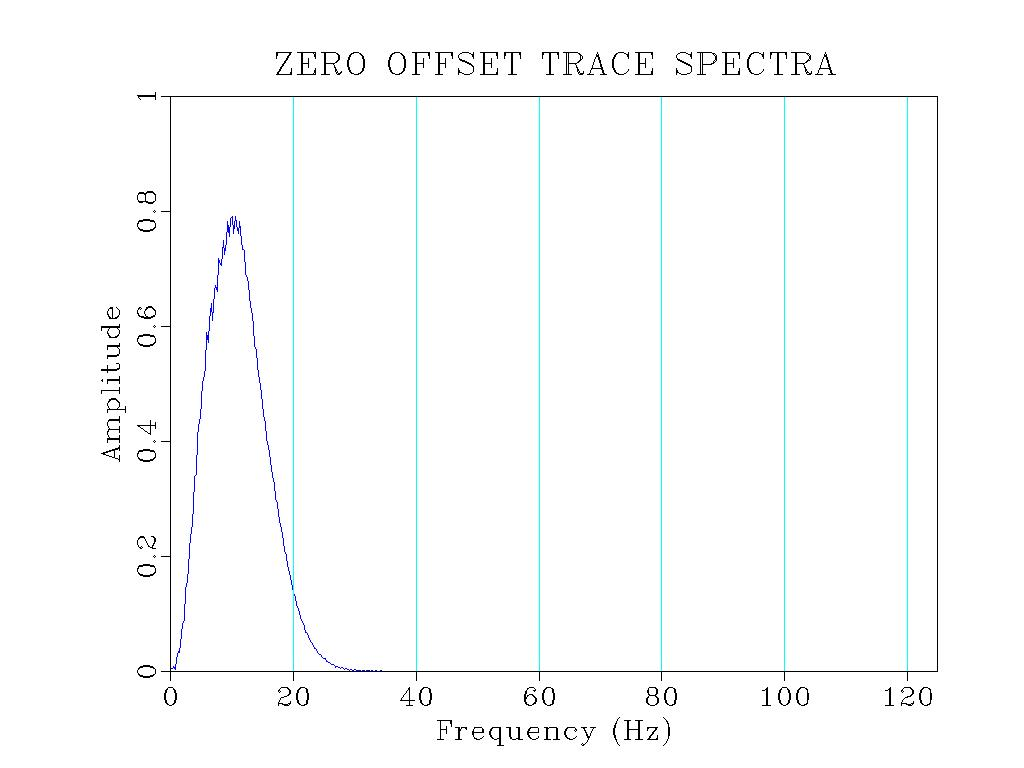
\includegraphics[scale=0.4]{images/originalTraceSpectra.jpeg}
\vspace{-0.3cm}
\end{center}
\begin{center}
 Fonte: Do Autor.
\end{center}
\label{fig:7.1}
\end{figure}


\begin{figure}
\caption{Resultado do empilhamento CRE: Supertraço para m0=4Km. A interpolação e o empilhamento cre adicionam
ruído numérico aos dados empilhados.}
\begin{center}
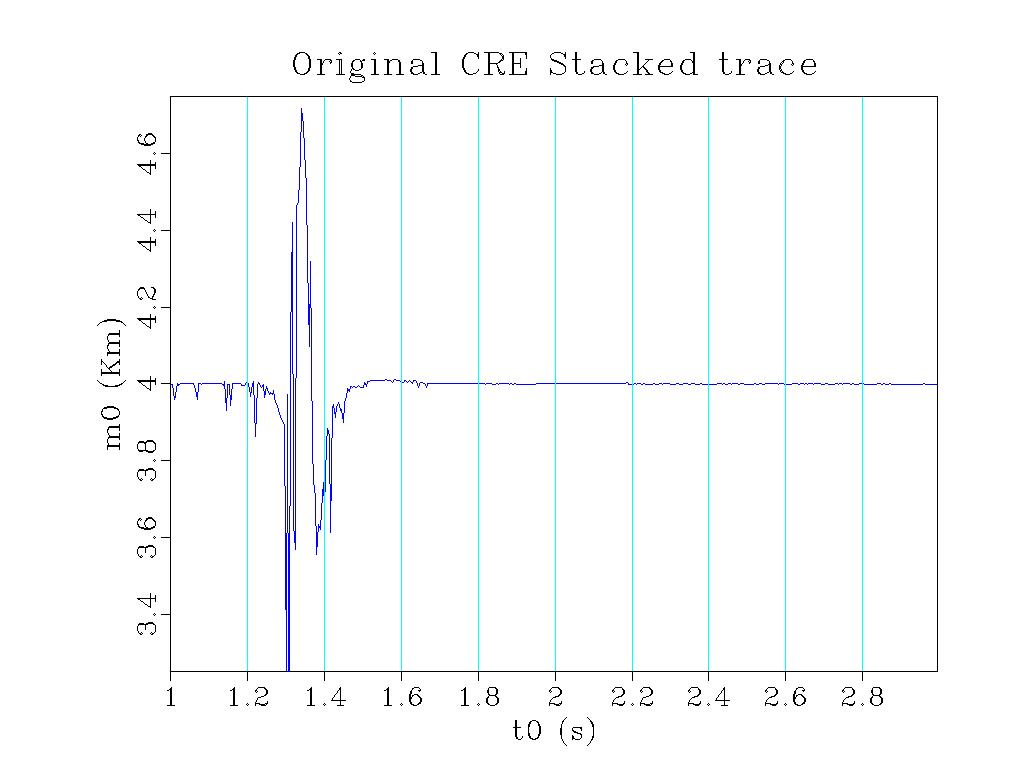
\includegraphics[scale=0.4]{images/creStackedSection.jpeg}
\vspace{-0.3cm}
\end{center}
\begin{center}
 Fonte: Do Autor.
\end{center}
\label{fig:7.2}
\end{figure}

\begin{figure}
\caption{Espectro de amplitude original do supertraço CRE para m0=4Km.}
\begin{center}
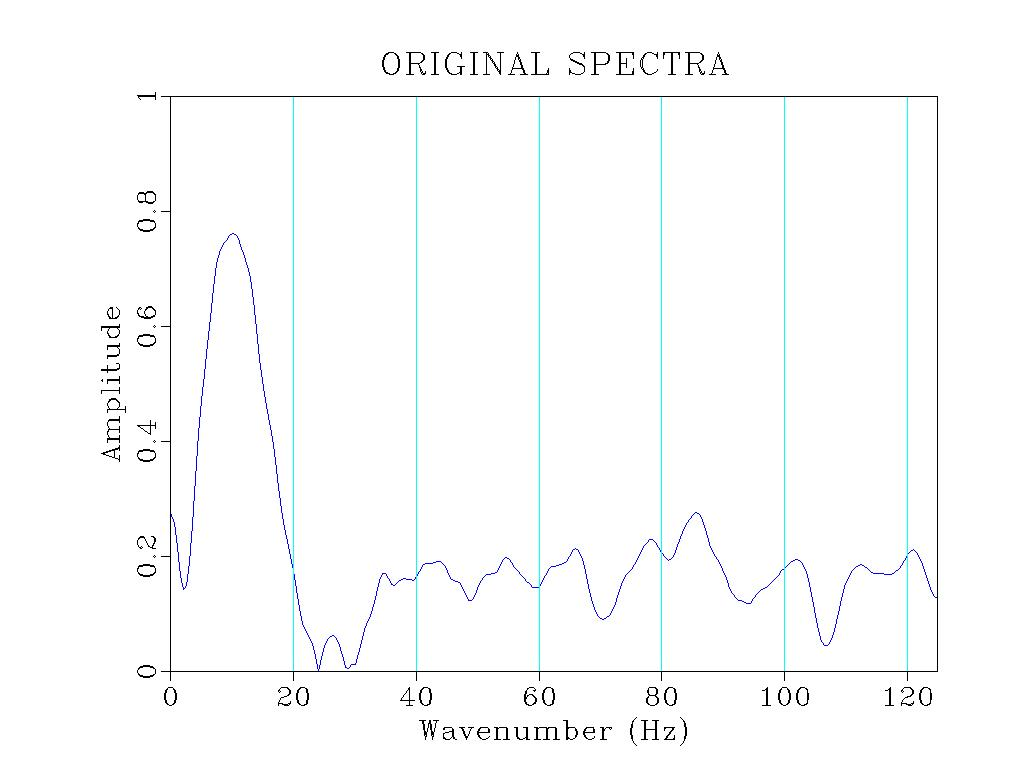
\includegraphics[scale=0.4]{images/originalSpectra.jpeg}
\vspace{-0.3cm}
\end{center}
\begin{center}
 Fonte: Do Autor.
\end{center}
\label{fig:7.3}
\end{figure}

\begin{figure}
\caption{Supertraço cre após a filtragem banda passante.}
\begin{center}
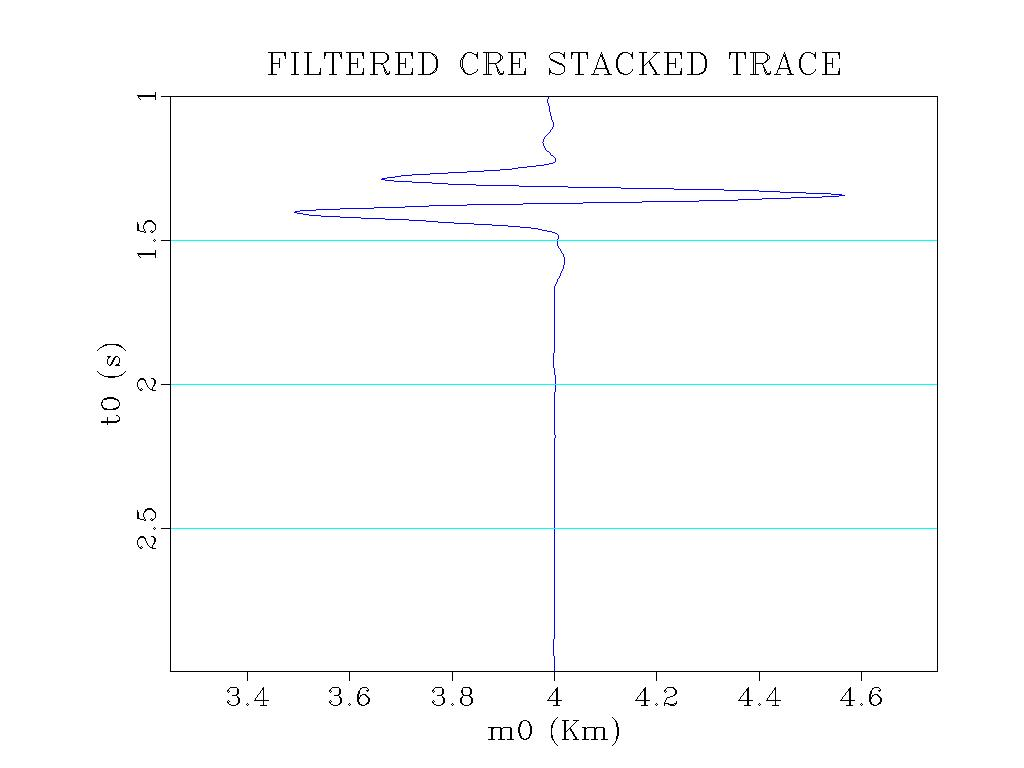
\includegraphics[scale=0.4]{images/creStackedSectionFiltered.jpeg}
\vspace{-0.3cm}
\end{center}
\begin{center}
 Fonte: Do Autor.
\end{center}
\label{fig:7.4}
\end{figure}

\begin{figure}
\caption{Espectro de amplitude após a filtragem banda passante.}
\begin{center}
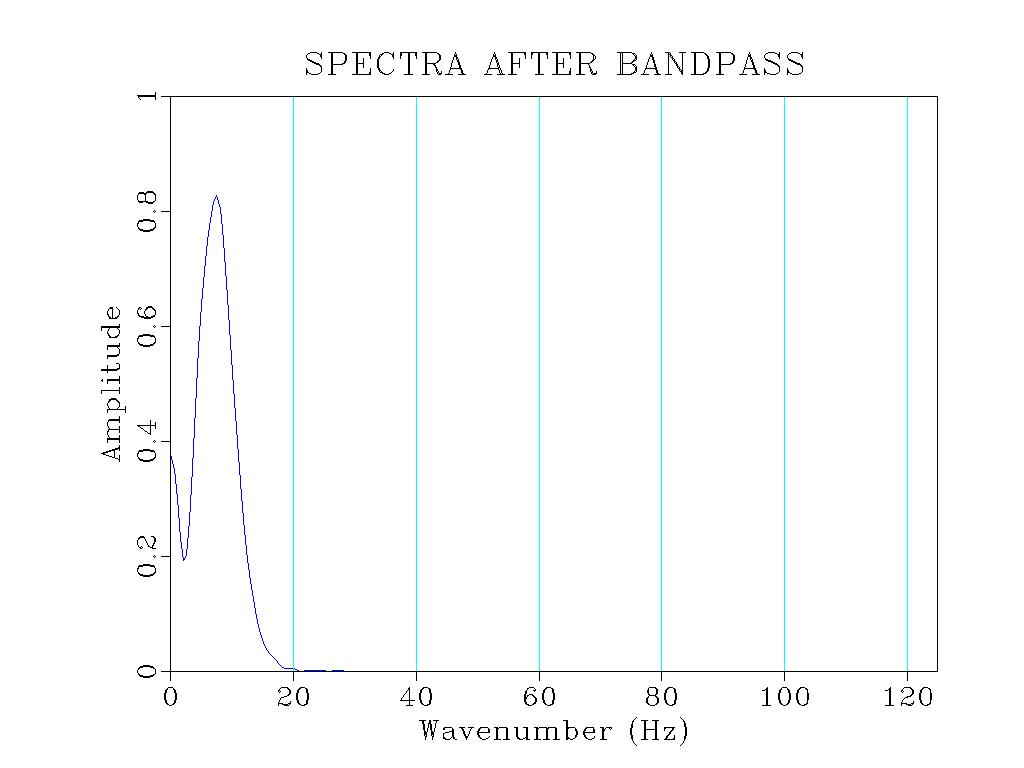
\includegraphics[scale=0.4]{images/filteredSpectra.jpeg}
\vspace{-0.3cm}
\end{center}
\begin{center}
 Fonte: Do Autor.
\end{center}
\label{fig:7.5}
\end{figure}

